%
% File main.tex
%

\documentclass[11pt]{article}
\usepackage{acl2016}
\usepackage{times}
\usepackage{latexsym}
\usepackage{float}

% \usepackage[utf8]{inputenc}
\usepackage{fontspec}
\usepackage{pgfplots}
\usepackage{tikz}
\pgfdeclarelayer{nodelayer}
\pgfdeclarelayer{edgelayer}
\pgfsetlayers{edgelayer,nodelayer,main}
\usetikzlibrary{arrows.meta}

\usepackage{graphicx}
\graphicspath{ {./img/} }

% math
\usepackage{amsmath}
\DeclareMathOperator*{\argmin}{arg\,min}
\DeclareMathOperator*{\argmax}{arg\,max}

\pgfplotsset{compat=1.12} 

% \renewcommand{\thefigure}{{\bf \arabic{figure}}}
% \renewcommand{\figurename}{{\bf Figure}}
%\renewcommand\labelitemi{--}

\aclfinalcopy % Uncomment this line for the final submission
%\def\aclpaperid{***} %  Enter the acl Paper ID here

% To expand the titlebox for more authors, uncomment
% below and set accordingly.
% \addtolength\titlebox{.5in}    

\newcommand\BibTeX{B{\sc ib}\TeX}

\title{Best Answer Prediction on Stack Overflow Data Set}

% Author information can be set in various styles:
% For several authors from the same institution:
% \author{Author 1 \and ... \and Author n \\
%         Address line \\ ... \\ Address line}
% if the names do not fit well on one line use
%         Author 1 \\ {\bf Author 2} \\ ... \\ {\bf Author n} \\
% For authors from different institutions:
% \author{Author 1 \\ Address line \\  ... \\ Address line
%         \And  ... \And
%         Author n \\ Address line \\ ... \\ Address line}
% To start a seperate ``row'' of authors use \AND, as in
% \author{Author 1 \\ Address line \\  ... \\ Address line
%         \AND
%         Author 2 \\ Address line \\ ... \\ Address line \And
%         Author 3 \\ Address line \\ ... \\ Address line}
% If the title and author information does not fit in the area allocated,
% place \setlength\titlebox{<new height>} right after
% at the top, where <new height> can be something larger than 2.25in
\author{Taikai Takeda\\
	    {\tt taikait@uci.edu}
	  \And
	Weicheng Yu\\
  {\tt weicheny@uci.edu}
  \And 
  Xingwei Liu \\
  {\tt xingweil@uci.edu}
  }

\date{}

\begin{document}

\maketitle

\begin{abstract}
Our project aims to automatically predict the most popular answer from a set of user-provided answers to a specific technical questions in Stack Overflow. We will use two different type of features: answer style and QA correlation. In terms of model, we concentrate on simple ones such as logistic regression because scalability matters. Our main contributions are 1) improved an accuracy score by adding various features, 2) found effective features that reflect characteristics of this specific data set.
\end{abstract}

\section{Introduction and Problem Statement}
For many people, Q\&A websites like Quora have become the go-to places when they run into problems. These websites usually keep track of how effective an answer is by counting the number of votes it receives from users. Higher votes usually means better quality. Reading some of the most popular answers on Stack Overflow, we wonder if there is a pattern in them. The motivation for this project was the idea of being able to "guess" the most popular answer to a problem without any support of knowledge base.

We will concentrate on Stack Overflow QA data set because it is technical QA. Most of previous work is focused on non-technical QA, for example, Baidu Zhidao ~\cite{Wang2010} and Yahoo! Answers ~\cite{Surdeanu2011,Qiu2015}. We believe that there are some inherent qualities of an answer to a technical question that make it popular among users. Our hypothesis is that a good answer should provide adequate information, be it text, images, hyperlinks, or code blocks. In addition, the quality of writing should also be an important factor because people tend to favor elegantly written answers over casually written ones. By experimenting different machine learning techniques, we hope to discover preferences of answers among Stack Overflow users.

\section{Related Work}
This task is called Community Question Answering (cQA). A lot of work has been done in this domain, which shows that it is quite an interesting problem in NLP. Some of the difficulties include retrieving answers for a new question from previous question-answer pairs ~\cite{Zhou2016}. Another difficulty comes from learning to rank answer candidates given a question, which is closely related to what we will do in this project.

Typically, only the best or the most popular answer is important for Q\&A. Hence, it is possible to not rank every answer.The traditional way to tackle this problem is to combine some features that seem to be useful for this task ~\cite{Surdeanu2011}. Recently, some other approaches have been tested out using Neural Network, which models correlation between questions and answers \cite{Tan2015,Qiu2015}.

\section{Data Sets}

Internet Archive\footnote{\small http://archive.org/download/stackexchange} provides archives questions and answers from StackOverflow. The original file  was in XML format. Every node in the file represents an entry of either a question or an answer. Every entry has the following fields, which are ID, number of up votes, parent ID, number of children, and the HTML formatted content. 

\subsection{Preprocessing Data}
As is usually the case, the data downloaded from the Internet are not organized in the format we want. We have to do some preprocessing in order to make the data easier to use. 
\subsubsection{Data Format}
The difficulty with the data-set is that is it was organized in a flat structure. As discussed above, the file we retrieved contains an array of entries of either question or answer in creation order. In this project, we need our data-set to be in pair of question-answer-set format, so we first preprocess the data into JSON format where keys are question ID and values are answers. Because the whole file is nearly 40GB, to save memory, we write a JSON file when 10,000 questions are processed.
\subsubsection{Data Reformatting}
We first wrote a python script to divide the file into 111 smaller files organized by answer numbers. From \texttt{Figure \ref{fig_a}}, we can see that the number of questions with a certain number of answers decrease rapidly as the number of answers increase. By organizing our data this way, we can easily pick out the data containing questions with a specific number of answers. One thing that is worth mentioning is that all the text contents of questions and answers are stored in HTML format, which means that there are many HTML tags in our data. Because we might need the pure text information, we wrote a number of utility functions to remove HTML tags in our data using Python regular expression and json libraries. Then we can feed the processed data to the NLTK library and start the feature extraction process.
\subsection{Statistical Information}
\begin{table}[H]
\centering
\begin{tabular}{ll}
\# of Question & 10789362  \\
\# of Answer   & 17650222 \\
Max \# of Ans  & 518      \\
Avg \# of Ans  & 1.64     
\end{tabular}
\end{table}

\begin{figure}[H]
\includegraphics[width=0.98\columnwidth]{dataset_stat.pdf}
\caption{\textbf{Answer Number Distribution}: \\ This figure shows the distribution of question numbers against questions of specific number of answers. }
\label{fig_a}
\end{figure}
\subsection{Normalization}
Another problem of the data-set is that the number of votes vary greatly depending on the attributes of the questions. For example, there are many questions that are very basic but are commonly asked. These questions tend to have best answers with a very large amount of up votes, because more people are concerned with the questions and they tend to have well-written answers. However, very technical and geeky questions tend not to get so much attention as there is a smaller amount of people who know and care about them. Hence, it is possible that even the highest voted answers have only a few up votes. The discrepancy creates problem in the actual training process because it will favor more commonly asked questions. Therefore, we need to regularize the votes so that all questions are trained under the same scale. The way we regularize the vote is to rescale the votes for each question by setting the highest voted answer to 1. Other answers will be set proportionally. 
\subsection{Train/Test Data}
To simplify the problem, we use the data-set of questions that have same number of answers. When train models, we splite the data-set by 75/25 into train and test data. Also, for hyperparameter optimization, we use the training set and do 3-fold cross validation to test the accuracy of different parameter configuration. 
% detail explanation about data
% In the original data, preference of is shown as the number of votes the answer got. However, since this measure differs from topic to topic, we regularize it by dividing by the maximum score within answers corresponding to the same question. 


\section{Description of Technical Approach}
\label{sec:tech}
Overall predictive model structure is illustrated in Figure~\ref{fig:model}. Generally speaking, there are two major components in it: features and models. Here, we will explain them in detail.
\begin{figure*}[t]
    \centering
	\tikzset{>={Latex[width=2mm,length=2mm]}}
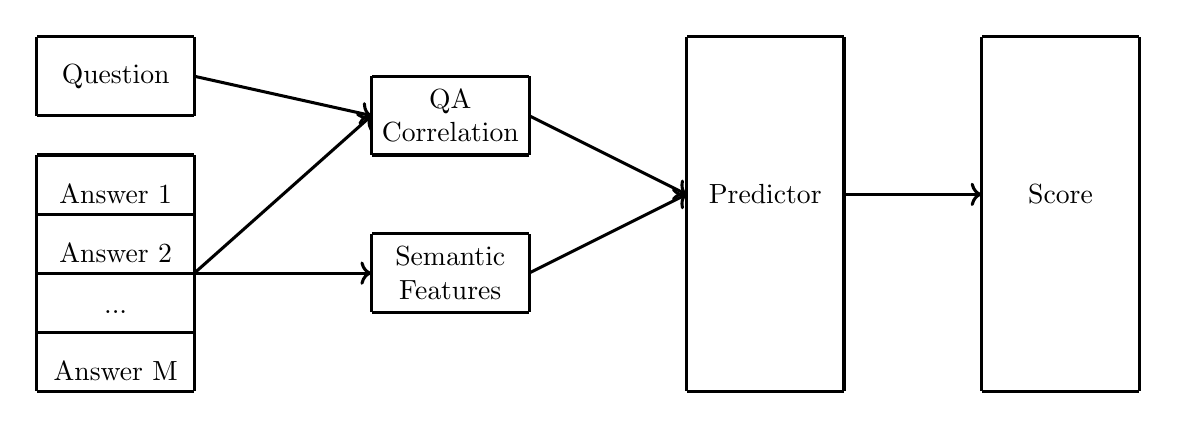
\begin{tikzpicture}
	\begin{pgfonlayer}{nodelayer}
		\node [] (0) at (-4.25, 4) {};
		\node [] (1) at (-4.25, 3) {};
		\node [] (2) at (-2.25, 3) {};
		\node [] (3) at (-2.25, 4) {};
		\node [] (4) at (-4.25, -0.5) {};
		\node [] (5) at (-2.25, -0.5) {};
		\node [] (6) at (-4.25, 2.5) {};
		\node [] (7) at (-2.25, 2.5) {};
		\node [] (8) at (-4.25, 1.75) {};
		\node [] (9) at (-2.25, 1.75) {};
		\node [] (10) at (-4.25, 1) {};
		\node [] (11) at (-2.25, 1) {};
		\node [] (12) at (-4.25, 0.25) {};
		\node [] (13) at (-2.25, 0.25) {};
		\node [] (14) at (0, 3.5) {};
		\node [] (15) at (0, 1.5) {};
		\node [] (16) at (0, 0.5) {};
		\node [] (17) at (2, 0.5) {};
		\node [] (18) at (2, 1.5) {};
		\node [] (19) at (0, 2.5) {};
		\node [] (20) at (2, 2.5) {};
		\node [] (21) at (2, 3.5) {};
		\node [] (22) at (4, 4) {};
		\node [] (23) at (4, -0.5) {};
		\node [] (24) at (6, -0.5) {};
		\node [] (25) at (6, 4) {};
		\node [] (26) at (9.75, 4) {};
		\node [] (27) at (7.75, 4) {};
		\node [] (28) at (7.75, -0.5) {};
		\node [] (29) at (9.75, -0.5) {};
		\node [] (30) at (0, 3) {};
		\node [] (31) at (0, 1) {};
		\node [] (32) at (4, 2) {};
		\node [] (33) at (7.75, 2) {};
		\node [] (34) at (-2.25, 3.5) {};
		\node [] (35) at (2, 3) {};
		\node [] (36) at (2, 1) {};
		\node [] (37) at (6, 2) {};
		\node [] (38) at (-3.25, 3.5) {Question};
		\node [] (39) at (-3.25, 2) {Answer 1};
		\node [] (40) at (-3.25, 1.25) {Answer 2};
		\node [] (41) at (-3.25, 0.5) {...};
		\node [] (42) at (-3.25, -0.25) {Answer M};
		\node [text width=2cm,align=center] (43) at (1, 3) {QA\\Correlation};
		\node [text width=2cm,align=center] (44) at (1, 1) {Semantic \\ Features};
		\node [] (45) at (5, 2) {Predictor};
		\node [] (46) at (8.75, 2) {Score};
	\end{pgfonlayer}
	\begin{pgfonlayer}{edgelayer}
		\draw [line width=1.1pt] (0.center) to (1.center);
		\draw [line width=1.1pt] (1.center) to (2.center);
		\draw [line width=1.1pt] (2.center) to (3.center);
		\draw [line width=1.1pt] (3.center) to (0.center);
		\draw [line width=1.1pt] (6.center) to (4.center);
		\draw [line width=1.1pt] (4.center) to (5.center);
		\draw [line width=1.1pt] (5.center) to (7.center);
		\draw [line width=1.1pt] (7.center) to (6.center);
		\draw [line width=1.1pt] (12.center) to (13.center);
		\draw [line width=1.1pt] (10.center) to (11.center);
		\draw [line width=1.1pt] (8.center) to (9.center);
		\draw [line width=1.1pt] (14.center) to (19.center);
		\draw [line width=1.1pt] (19.center) to (20.center);
		\draw [line width=1.1pt] (20.center) to (21.center);
		\draw [line width=1.1pt] (21.center) to (14.center);
		\draw [line width=1.1pt] (15.center) to (16.center);
		\draw [line width=1.1pt] (16.center) to (17.center);
		\draw [line width=1.1pt] (17.center) to (18.center);
		\draw [line width=1.1pt] (18.center) to (15.center);
		\draw [line width=1.1pt] (22.center) to (23.center);
		\draw [line width=1.1pt] (23.center) to (24.center);
		\draw [line width=1.1pt] (24.center) to (25.center);
		\draw [line width=1.1pt] (25.center) to (22.center);
		\draw [line width=1.1pt] (27.center) to (28.center);
		\draw [line width=1.1pt] (28.center) to (29.center);
		\draw [line width=1.1pt] (29.center) to (26.center);
		\draw [line width=1.1pt] (26.center) to (27.center);
		\draw [->,line width=1.1pt] (11.center) to (30.center);
		\draw [->,line width=1.1pt] (11.center) to (31.center);
		\draw [->,line width=1.1pt] (34.center) to (30.center);
		\draw [->,line width=1.1pt] (35.center) to (32.center);
		\draw [->,line width=1.1pt] (36.center) to (32.center);
		\draw [->,line width=1.1pt] (37.center) to (33.center);
	\end{pgfonlayer}
\end{tikzpicture}
    %\includegraphics[width=\textwidth]{pipeline_pp.pdf}
    \caption{{\bf Predictive Model}: Answer style and QA correlation are two different type of features. With these features, predictor produces predicted scores. An answer with maximum score is predicted as the best answer.}
    \label{fig:model}
\end{figure*}

\subsection{Preliminary}
Here, we will introduce notations. Let question set be $Q = \{q^1,\cdots, q^N\}$ where $N$ is the number of questions in data set. Similarly, let answer set be $A = \{a^1,\cdots,a^N \}$ where each $a^i$ is sequence of answer candidates $a^i = (a^i_1, \cdots , a^i_M)$. We fixed the number of answer candidates $M$ because we cannot directly compare the result with different $M$. Target is denoted as $T=\{t^1, \cdots, t^N\}$. Each $t^i$ is $M-$length sequence of answer score, $t^i = (t^i_1, \cdots ,t^i_M)$ where $t^i_j \in [0,1]$. True label set $Y$ is $Y=\{y^1, \cdots, y^N\}$ where $y^i \in \{1, \cdots , M\}$ is label of the best answers $y^i = \argmax_{j} t^i_j$, i.e. $y^i$-th answer $a^i_{y^i}$ is the best answer for $q^i$. Our goal is to obtain good prediction function $f: Q \times A \rightarrow \{1,\cdots , M\}$. Evaluation measure that shows goodness of this predictor is explained in the next subsection.

\subsection{Evaluation Measure}
We employ Re-ranking Precision at 1st position (P@1) as an evaluation measure, since we are interested mainly in the best answer. We divide the number of correctly predicted answers by the total number of QA pairs. The fraction represents the accuracy of our prediction for the best answer. 
\begin{eqnarray}
P@1=\frac{\#\{\mbox{\small correctly re-ranked into the first position}\}}{\#\{\mbox{\small all QA pairs}\}} \nonumber
\end{eqnarray}
More formally, 
\begin{eqnarray}
P@1=\frac{\sum_{i=1}^N I(f(q^i, a^i) = y^i)}{N}\nonumber
\end{eqnarray}
where $I$ is indicator function. Clearly, this measure largely depends on the number of answer candidates $M$, so we used fixed $M \in \{2,5,10,15,20\}$ for evaluation purpose.

\subsection{Features}

In terms of extracting features, we tried two different approaches: one is to analyze answer documents independently, and the other is to capture correlation between questions and answers.  Since these two factors are orthogonal, we combine both features using these two different approaches and feed them to predictive models. Here, we will explain these two approaches separately.

\subsection{Answer Style Analysis}
We assume that good answers exhibits a similar style. For example, an answer with lots of casual and informal words is not likely to be favored by users. In contrast, an answer with correct grammar and formal vocabulary is likely to get a vote up. Hence, even if we do not know what the original question is, we can find a "better" answer.  Here, we are going to model the preference of answers in the following ways:
\begin{itemize}
\setlength\itemsep{0em}
\item \textbf{BoW:}
\\Use the basic Bag of Words as a feature to train our models.
\item \textbf{Sentence Counts Heuristic:}
\\Choose the best answer based on the number of sentences an answer has. The answer with the most counts is the best.
\item \textbf{HTML Tags:}
\\Since the answers we get are embeded in HTML, we can choose either to pass in the whole HTML objects as input or to extract only text answers as input. 
\item \textbf{Heuristic:}
\\We build some simple heuristic methods to explore possible features for our machine learning models. Those heuristic functions are based on number of characters, number of words, number of sentences, and average sentence length. For some of them, we also have an additional version that up-weighs code block's length (UWC) to capture the importance of the code blocks. 

\end{itemize}


\subsection{Correlation between Question and Answer}
Correlation between questions and answers is another concern. A good answer should responds directly to the question. Therefore, modeling this correlation should be helpful to find the best answer. However, modeling the correlation is not trivial. The first approach is to compute a similarity score between question and answer documents. We vectorize them with BoW, and project them onto hidden space using Latent Semantic Analysis (LSA). Then, we compute cosine similarity of them and use it as a feature.

\subsection{Predictive Models}
We picked some models because characteristics of the model can make a difference. Also, we tried both regression models and classification models because binarizing the score might affect our results. For classification models, target value is binarized with threshold set to $1.0$, which means that only the best answers are labeled as $1$. Indeed, there would be the room to optimize this threshold, so we will do it in hyper parameter tuning, which is planned to be done in 9th week.  We did not choose non-linear models because it takes much more time to optimize (e.g. RBF-SVM).

\section{Software}

We share all the code on GitHub \footnote{{\small https://github.com/bigsea-t/best-answer-prediction}}

The primary software we use is Python version 3.5. Our code are majorly written in python with NLTK  as tokenization library and scikit-learn as the machine learning library. \textit{Main.py} runs the predictor and produce the accuracy results. \textit{Preprocess.py} divides data by the number of answers. \textit{Others} are some helpers to transform data and process text.

We wrote all other Python code for this project by ourselves.
\section{Experiments and Evaluation}
Here, we will show our experiment results. 

\subsection{Accuracy Scores}
We added various features to the basic models. First, we added QA correlation feature, then mixed heuristic features. Here, we will show result for each one.

\begin{table}[t]
\centering
\begin{tabular}{r|ccccl}
\multicolumn{1}{l|}
	{\small{\textbf{\# Ans}}}  & \textbf{LSVM} & \textbf{LoR} & \textbf{RiR} & \textbf{LiR} \\
    \cline{1-5}
    \textbf{2}  
    & \begin{tabular}[c]{@{}c@{}}61.23\\ \textit{69.17} \\ 69.06 \\ 61.51\end{tabular} 
    & \begin{tabular}[c]{@{}c@{}}\textbf{61.28}\\ \textbf{\textit{69.28}} \\ \textbf{69.15} \\ \textbf{61.54} \end{tabular} 
    & \begin{tabular}[c]{@{}c@{}}61.19\\ 68.97 \\ \textit{69.01} \\ 61.49 \end{tabular} 
    & \begin{tabular}[c]{@{}c@{}}59.45\\ \textit{66.96 }\\ 66.89 \\ 59.60 \end{tabular} 
    & \begin{tabular}[l]{@{}l@{}} \small{(!tag, !cor)} \\ \small{(tag, !cor)} \\ \small{(tag, cor)} \\ \small{(!tag, cor)} \end{tabular}\\ 
    \cline{1-5}
    \textbf{5}            
    & \begin{tabular}[c]{@{}c@{}}30.81\\ \textbf{43.47} \\ \textbf{\textit{43.50}} \\ 30.81 \end{tabular} 
    & \begin{tabular}[c]{@{}c@{}}\textbf{30.96}\\ 43.29 \\ \textit{43.38 }\\ \textbf{30.83}\end{tabular} 
    & \begin{tabular}[c]{@{}c@{}}30.62\\ 42.96 \\ \textit{43.12} \\ 30.76\end{tabular} 
    & \begin{tabular}[c]{@{}c@{}}27.32\\ 40.37 \\ 40.44 \\ 27.52 \end{tabular} \\ 
    \cline{1-5}
	\textbf{10}           
	& \begin{tabular}[c]{@{}c@{}}17.52\\ 30.49 \\ \textbf{\textit{30.69}} \\ 18.54 \end{tabular} 
    & \begin{tabular}[c]{@{}c@{}}18.05\\ 30.15 \\ \textit{30.20} \\ 18.49 \end{tabular} 
    & \begin{tabular}[c]{@{}c@{}}\textbf{18.49}\\ \textit{\textbf{30.83}}\\ 30.35 \\ \textbf{19.36} \end{tabular} 
    & \begin{tabular}[c]{@{}c@{}}15.49\\ \textit{27.40}\\ 26.57 \\ 15.34 \end{tabular} \\ 
    \cline{1-5}
	\textbf{15}           
    & \begin{tabular}[c]{@{}c@{}}12.83\\ \textit{22.77} \\ 20.68 \\ 13.61 \end{tabular} 
    & \begin{tabular}[c]{@{}c@{}}13.35\\ 22.51 \\ \textbf{\textit{24.08}} \\ \textbf{15.18} \end{tabular} 
    & \begin{tabular}[c]{@{}c@{}}\textbf{16.75}\\ \textbf{23.04} \\ \textit{23.56} \\ 13.87\end{tabular} 
    & \begin{tabular}[c]{@{}c@{}}13.09\\ \textit{21.73} \\ 19.63 \\ 11.26\end{tabular} \\ 
    \cline{1-5}
	\textbf{20}           
    & \begin{tabular}[c]{@{}c@{}}7.76\\ 14.66 \\ \textbf{\textit{16.38}} \\ \textbf{8.62} \end{tabular} 
    & \begin{tabular}[c]{@{}c@{}}\textbf{8.62}\\ 13.79 \\ \textit{14.66} \\ 6.03\end{tabular} 
    & \begin{tabular}[c]{@{}c@{}}6.90\\ \textit{\textbf{15.52}} \\ 14.66 \\ \textbf{8.62}\end{tabular} 
    & \begin{tabular}[c]{@{}c@{}}6.03\\ \textit{13.79} \\ 12.07 \\ \textbf{8.62}\end{tabular}
\end{tabular}
\caption{\textbf{P@1 accuracy scores for Linear SVM, Logistic Regression, Ridge Regression and Linear Regression}: \textbf{bold} numbers mean the best result of four models given a  number of answers on a feature processing configuration.  \textit{italicized} numbers mean the best result of a model among all feature processing configurations on a number of answers. \texttt{!tag} means removing tags. \texttt{tag} means keeping tags. \texttt{col} means using cosine distance between answers and questions in latent semantic space as a feature (q-a correlation). \texttt{!col} means not using q-a correlation as a feature.}
\label{tab_accuracy}
\end{table}

\begin{table}
\centering
\begin{tabular}{r|cc}
\textbf{Methods}          & \textbf{Default}                                      & \textbf{UWC}                               \\ \hline
\textbf{Original}           & \begin{tabular}[c]{@{}c@{}}32.22\\ 30.20\end{tabular} & N/A                                                   \\ \hline
\textbf{\# Char}          & \begin{tabular}[c]{@{}c@{}}32.48\\ 30.45\end{tabular} & \begin{tabular}[c]{@{}c@{}}32.03\\ 30.83\end{tabular} \\ \hline
\textbf{\# Word}          & \begin{tabular}[c]{@{}c@{}}32.41\\ 30.98\end{tabular} & N/A                                                   \\ \hline
\textbf{\# Sent}      & \begin{tabular}[c]{@{}c@{}}32.48\\ 31.46\end{tabular} & \begin{tabular}[c]{@{}c@{}}32.46\\ 31.56\end{tabular} \\ \hline
\textbf{\# W/S} & \begin{tabular}[c]{@{}c@{}}32.28\\ 30.45\end{tabular} & N/A                                                  
\end{tabular}
\caption{\textbf{Heuristic mix-model accuracy:}\\ The train and test accuracy of mixed model of logistic regression and heuristic methods}
\label{tab:acc_mix}
\end{table}


The accuracy result of adding QA correlation and html tags is shown in \texttt{Table \ref{tab_accuracy}}. We can say from this result 1) the number of answers significantly influences the accuracy as expected. 
2) For a given model and a specific answer configuration(whether we keep the HTML tags and whether we take QA correlation into consideration), keeping the HTML tags in the tokenization phase significantly improves the accuracy results in all models.
3) Logistic regression and ridge regression produce slightly more accurate predictions under the same configuration. 
4) The first three models work relatively well and all produce close results. However, linear regression exhibits some deficiencies in the prediction. 
5) Taking QA distance into consideration does not produce a distinguishable difference in the prediction result. 

We also added heuristic features. We set up some mixed models that use the output of heuristic functions as additional features to logistic regression model. We tested them in 10-answer data-set. The result is shown in \texttt{Table \ref{tab:acc_mix}}.
Here, we show how adding heuristic features affects the result.
There is also no difference between up-weighing code block and the normal weighing method. This is because logistic regression using bag of words method already extracts the information of code blocks from text. In addition, incorporating heuristic functions to machine learning models only increases less than one percent of test accuracy.

\subsection{Hyper-Parameter Optimization}
We exploited random search on Hyper-Parameter Optimization  \cite{Bergstra2012} rather than grid search.  We tried 50 iterations for every model's parameter space and chose the 5 best configurations  from each model according to their validation score.  We tested on the 10-answer data-set with all selected configurations on our models. The result is shown in \texttt{Table \ref{tab:hpo}}.

\begin{table}[t]
\centering
\begin{tabular}{r|cccc}
\multicolumn{1}{l|}{\textbf{Rank}} & \textbf{LSVM}                                                  & \textbf{LoR}                                                   & \textbf{RiR}                                                   & \textbf{LiR}                                                   \\ \hline
\textbf{default}                   & \begin{tabular}[c]{@{}c@{}}32.27\\ 30.49\end{tabular}          & \begin{tabular}[c]{@{}c@{}}32.22\\ 30.15\end{tabular}          & \begin{tabular}[c]{@{}c@{}}31.06\\ 30.83\end{tabular}          & \begin{tabular}[c]{@{}c@{}}29.28\\ 27.40\end{tabular}          \\ \hline
\textbf{1}                         & \textbf{\begin{tabular}[c]{@{}c@{}}32.14\\ 30.69\end{tabular}} & \begin{tabular}[c]{@{}c@{}}32.12\\ 30.11\end{tabular}          & \begin{tabular}[c]{@{}c@{}}32.11\\ 30.88\end{tabular}          & \textbf{\begin{tabular}[c]{@{}c@{}}32.07\\ 30.54\end{tabular}} \\ \hline
\textbf{2}                         & \begin{tabular}[c]{@{}c@{}}32.20\\ 30.35\end{tabular}          & \textbf{\begin{tabular}[c]{@{}c@{}}32.19\\ 30.20\end{tabular}} & \begin{tabular}[c]{@{}c@{}}32.12\\ 30.93\end{tabular}          & \begin{tabular}[c]{@{}c@{}}32.07\\ 30.54\end{tabular}          \\ \hline
\textbf{3}                         & \begin{tabular}[c]{@{}c@{}}32.20\\ 30.35\end{tabular}          & \begin{tabular}[c]{@{}c@{}}32.24\\ 30.15\end{tabular}          & \begin{tabular}[c]{@{}c@{}}32.11\\ 30.88\end{tabular}          & \begin{tabular}[c]{@{}c@{}}30.27\\ 27.78\end{tabular}          \\ \hline
\textbf{4}                         & \begin{tabular}[c]{@{}c@{}}32.20\\ 30.35\end{tabular}          & \begin{tabular}[c]{@{}c@{}}32.17\\ 30.06\end{tabular}          & \textbf{\begin{tabular}[c]{@{}c@{}}32.11\\ 30.98\end{tabular}} & \begin{tabular}[c]{@{}c@{}}30.27\\ 27.78\end{tabular}          \\ \hline
\textbf{5}                         & \begin{tabular}[c]{@{}c@{}}11.92\\ 11.47\end{tabular}          & \begin{tabular}[c]{@{}c@{}}31.91\\ 29.72\end{tabular}          & \begin{tabular}[c]{@{}c@{}}32.12\\ 30.88\end{tabular}          & \begin{tabular}[c]{@{}c@{}}N/A\\ N/A\end{tabular}             
\end{tabular}
\caption{\textbf{Hyper-Parameter Optimization Result}: The result of hyper-parameter optimization. Rank shows the rank of accuracy on validation set, e.g. rank 1 is the best configuration according to the random search. `default' is the score before optimization. The first row of each rank is training accuracy, and the second is test accuracy. The best test accuracy results are bold.}
\label{tab:hpo}
\end{table}

From this result, we conclude that because of the simplicity of linear models, the hyper parameters do not affect the result in a significant way. Only linear regression models have noticeable improvement when applied hyper parameter optimization. The difference in terms of the parameter choice is influenced by the intercept parameter, which means whether the data are centralized. In addition, we propose that the reason of discrepancy is a result of the data distribution, which is closer to origin in hyper space.
Details about the parameter type and range and the result are in code. 

\subsection{Overfitting}
\begin{figure}[t]
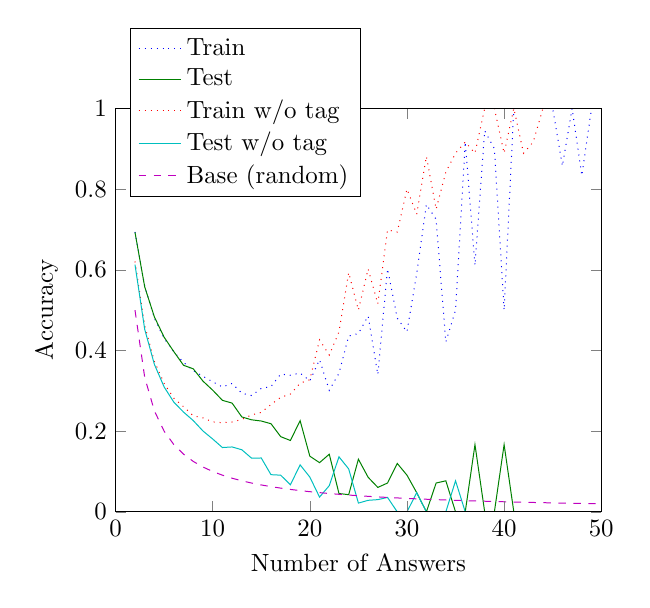
\begin{tikzpicture}[scale=0.9]

\definecolor{color1}{rgb}{0.75,0,0.75}
\definecolor{color0}{rgb}{0,0.75,0.75}

\begin{axis}[
xlabel={Number of Answers},
ylabel={Accuracy},
xmin=0, xmax=50,
ymin=0, ymax=1,
axis on top,
legend entries={{Train},{Test},{Train w/o tag},{Test w/o tag},{Base (random)}},
legend cell align={left},
legend style={at={(0.03,1.2)}, anchor=north west}
]
\addplot [blue, dotted]
table {%
2 0.693607037799778
3 0.559152712179762
4 0.47980443204497
5 0.429671047854186
6 0.396695648403114
7 0.370371788490255
8 0.350050851767099
9 0.336004162330905
10 0.322200709906421
11 0.309574217831099
12 0.318306010928962
13 0.293885601577909
14 0.288339670468948
15 0.305944055944056
16 0.310502283105023
17 0.341426403641882
18 0.338775510204082
19 0.344036697247706
20 0.324712643678161
21 0.377049180327869
22 0.301310043668122
23 0.343589743589744
24 0.435714285714286
25 0.442028985507246
26 0.485436893203884
27 0.34020618556701
28 0.602409638554217
29 0.48
30 0.446153846153846
31 0.590163934426229
32 0.761904761904762
33 0.725
34 0.421052631578947
35 0.5
36 0.916666666666667
37 0.611111111111111
38 0.944444444444444
39 0.9
40 0.5
41 1
42 1
43 1
44 1
45 1
46 0.857142857142857
47 1
48 0.833333333333333
49 1
50 1
51 1
52 1
53 1
54 1
55 1
56 1
57 1
58 1
61 1
62 1
64 1
65 1
67 1
68 1
69 1
70 1
71 1
72 1
73 1
78 1
87 1
100 1
129 0.5
};
\addplot [green!50.0!black]
table {%
2 0.692802024663176
3 0.557706462534962
4 0.482887922104827
5 0.432886758886105
6 0.397033953427865
7 0.363197794624397
8 0.354500381388253
9 0.323970037453184
10 0.301548886737657
11 0.276445698166432
12 0.269467213114754
13 0.235207100591716
14 0.228136882129278
15 0.225130890052356
16 0.218430034129693
17 0.186363636363636
18 0.176829268292683
19 0.226027397260274
20 0.137931034482759
21 0.121951219512195
22 0.142857142857143
23 0.0454545454545455
24 0.0425531914893617
25 0.130434782608696
26 0.0857142857142857
27 0.0606060606060606
28 0.0714285714285714
29 0.12
30 0.0909090909090909
31 0.0476190476190476
32 0
33 0.0714285714285714
34 0.0769230769230769
35 0
36 0
37 0.166666666666667
38 0
39 0
40 0.166666666666667
41 0
42 0
43 0
44 0
45 0
46 0
47 0
48 0
49 0
50 0
51 0
52 0
53 0
54 0
55 0
56 0
57 0
58 0
61 0
62 0
64 0
65 0
67 0
68 0
69 0
70 0
71 0
72 0
73 0
78 0
87 0
100 0
129 0
};
\addplot [red, dotted]
table {%
2 0.620554852547508
3 0.461563311455969
4 0.372559716592201
5 0.318362258853146
6 0.281607077036491
7 0.260519967837041
8 0.238176964149504
9 0.232882414151925
10 0.22297515327525
11 0.220889202540579
12 0.222677595628415
13 0.229289940828402
14 0.240177439797212
15 0.246503496503497
16 0.265981735159817
17 0.283763277693475
18 0.291836734693878
19 0.318807339449541
20 0.327586206896552
21 0.426229508196721
22 0.388646288209607
23 0.446153846153846
24 0.592857142857143
25 0.5
26 0.601941747572815
27 0.515463917525773
28 0.698795180722892
29 0.693333333333333
30 0.8
31 0.737704918032787
32 0.880952380952381
33 0.75
34 0.842105263157895
35 0.888888888888889
36 0.916666666666667
37 0.888888888888889
38 1
39 1
40 0.888888888888889
41 1
42 0.888888888888889
43 0.916666666666667
44 1
45 1
46 1
47 1
48 1
49 1
50 1
51 0.833333333333333
52 1
53 1
54 1
55 1
56 1
57 1
58 1
61 1
62 1
64 1
65 1
67 1
68 1
69 1
70 1
71 1
72 1
73 1
78 1
87 1
100 1
129 1
};
\addplot [color0]
table {%
2 0.612807979554872
3 0.452463320084401
4 0.365299357779159
5 0.309552336346803
6 0.27182255756472
7 0.247185848839881
8 0.226163234172387
9 0.200374531835206
10 0.18054211035818
11 0.159379407616361
12 0.160860655737705
13 0.153846153846154
14 0.133079847908745
15 0.133507853403141
16 0.0921501706484642
17 0.0909090909090909
18 0.0670731707317073
19 0.116438356164384
20 0.0862068965517241
21 0.0365853658536585
22 0.0649350649350649
23 0.136363636363636
24 0.106382978723404
25 0.0217391304347826
26 0.0285714285714286
27 0.0303030303030303
28 0.0357142857142857
29 0
30 0
31 0.0476190476190476
32 0
33 0
34 0
35 0.0769230769230769
36 0
37 0
38 0
39 0
40 0
41 0
42 0
43 0
44 0
45 0
46 0
47 0
48 0
49 0
50 0
51 0
52 0
53 0
54 0
55 0
56 0
57 0
58 0
61 0
62 0
64 0
65 0
67 0
68 0
69 0
70 0
71 0
72 0
73 0
78 0
87 0
100 0
129 0
};
\addplot [color1, dashed]
table {%
2 0.5
3 0.333333333333333
4 0.25
5 0.2
6 0.166666666666667
7 0.142857142857143
8 0.125
9 0.111111111111111
10 0.1
11 0.0909090909090909
12 0.0833333333333333
13 0.0769230769230769
14 0.0714285714285714
15 0.0666666666666667
16 0.0625
17 0.0588235294117647
18 0.0555555555555556
19 0.0526315789473684
20 0.05
21 0.0476190476190476
22 0.0454545454545455
23 0.0434782608695652
24 0.0416666666666667
25 0.04
26 0.0384615384615385
27 0.037037037037037
28 0.0357142857142857
29 0.0344827586206897
30 0.0333333333333333
31 0.032258064516129
32 0.03125
33 0.0303030303030303
34 0.0294117647058824
35 0.0285714285714286
36 0.0277777777777778
37 0.027027027027027
38 0.0263157894736842
39 0.0256410256410256
40 0.025
41 0.024390243902439
42 0.0238095238095238
43 0.0232558139534884
44 0.0227272727272727
45 0.0222222222222222
46 0.0217391304347826
47 0.0212765957446809
48 0.0208333333333333
49 0.0204081632653061
50 0.02
51 0.0196078431372549
52 0.0192307692307692
53 0.0188679245283019
54 0.0185185185185185
55 0.0181818181818182
56 0.0178571428571429
57 0.0175438596491228
58 0.0172413793103448
61 0.0163934426229508
62 0.0161290322580645
64 0.015625
65 0.0153846153846154
67 0.0149253731343284
68 0.0147058823529412
69 0.0144927536231884
70 0.0142857142857143
71 0.0140845070422535
72 0.0138888888888889
73 0.0136986301369863
78 0.0128205128205128
87 0.0114942528735632
100 0.01
129 0.00775193798449612
};
\end{axis}

\end{tikzpicture}
\caption{\textbf{Dynamics of Accuracy}: The performance  of Logistic Regression model on data-sets with different number of answers (without q-a correlation as feature). }
\label{fig_acc}
\end{figure}
In \texttt{Figure \ref{fig_acc}}, we show the train and test error for different number of answers. We see that the performance of our model is relatively stable for answers with number of questions under 15, and train error and test error are close. However, as we evaluate on questions with a larger number of answers, the performance deteriorates drastically, with test accuracy rapidly approaching 0 and train accuracy rapidly approaching 1. As we have shown in \texttt{Figure \ref{fig_a}}, the number of questions shrinks exponentially in  response to the increase of number of answers. As we have shown in the data-set section, the average number of answers a question has is 1.64.   Therefore, the increasing gap between train and test error, we believe, is the consequence of the over-fitting effect, which is caused by the reduced size of data-set.

\subsection{Effective Features}
Here, we will show which features are highly effective in terms of prediction. We only show the result about logistic regression because all the model have similar accuracy result. We can easily interpret this model by looking at the weight: larger weight means positive features , and smaller weight means negative features. Here are resulting top-10 most effective and least effective features:
\begin{description}
\setlength\itemsep{0em}
\item[\bf{Positive}] \hfill\\
edit, note, update equivalent, jsfiddle, finally, fact, instead, documentation, fix
\item[\bf{Negative}] \hfill\\
answers, think, tried, hope, maybe, answer, thought, guess, said, mentioned
\end{description}
Generally, positive features include {\it formal} words such as ``finally'' and ``fact'', and words that indicate {\it edit frequency} of an answer such as ``edit'' and ``update'' (Figure \ref{fig:edit} is typical example of an answer which include the word ``edit''). This result reveals that formal and eagerly edited answers are likely to be the best answers. On the other hand, negative features are more {\it ambiguous} words such as ``maybe'' and ``guess'' and words that {\it refer another answers} such as ``answers'' and ``said'' (Figure \ref{fig:answers} is typical example of an answer which include the word ``answers''). This shows that being ambiguous and referring another answer have negative effect in receiving more votes. \\
Interestingly, if we choose to keep the HTML tags, we find some additional top features  "href", "hr", "code", and "li", which have higher scores than the previously mentioned words. Our assumption is that  rich text elements increase credibility of answers because these links usually redirects to websites that are highly credible or focuses on a very specific domain of problems. 
\begin{figure}[t]
    \centering
	\includegraphics[width=0.98\columnwidth]{edit.pdf}
    \caption{{\bf Typical High-voted Answer}: Example of preferred answer with the word ``edit''. This word is an indicator of updated answer. }
    \label{fig:edit}
\end{figure}

\begin{figure}[t]
    \centering
	\includegraphics[width=0.98\columnwidth]{answers.pdf}
    \caption{{\bf Typical Low-voted Answer}: Example of preferred answer with the word ``answers''. It shows the world ``answer'' refers other answers.}
    \label{fig:answers}
\end{figure}

\section{Discussion and Conclusion}
In this project, we explored some feature extraction methods and predictive models for the Q\&A problem taken from StackExchange. We digged into every part of our model building process and tried different approaches in selecting functions and parameters. As a result, we were able to generate a large number of results reflecting how each selection affects our model accuracy. According to our results, on the one hand, choosing different predictive models does not yield a significantly different result. On the other hand, the ways in which we do feature extraction have a significant impact on the accuracy result. We also find that correlation between Q\&A using latent semantic analysis does not affect a lot. We conclude that question answer correlation, at least on vocabulary space, does not  make a difference in terms of answer popularity. Because of the fact that choosing good feature extraction technique yields much better result, in order to improve the performance of our model, we can try more advanced feature extraction techniques of document such as paragraph2vec or POS information. 

In addition to getting accuracy results, we also obtain some effective features of this specific data set. These features give us insights of what a good answer looks like. Being able to interpret some of our results is actually an advantage of choosing simpler model over complex model since it only reveals more obvious traits of our data-set. It also has the advantage of having less scalability issue than complex models.
% \section*{Acknowledgments}
% Thanks a lot for...

\bibliography{ref}
\bibliographystyle{acl2016}

\end{document}
